\chapter{Introduction}
\label{sec:intro}

Ever since the development of modern Computer Graphics, one of the goals 
researchers aspired to was being able to synthesize images indistinguishable 
from real photographs. In order to produce physically accurate images, the 
process of image synthesis - also called \textbf{rendering} - simulates the 
interaction of light with the representation of a three-dimensional scene. 

\textbf{Physically-Based Rendering (PBR)} is a complex process that requires 
thorough knowledge of optics, material properties, geometry and light 
propagation.

\section{Physically Based Rendering (PBR)}
PBR is implemented using Monte Carlo (MC) Ray Tracing \cite{Lafortune96mathematicalmodels}, which uses MC 
Integration \cite{Keller:2007} to estimate the environment illumination function 
by tracing (or sampling) the path of several light rays starting from an image 
plane, simulating the effects obtained from its encounters with virtual objects. 
While able to produce a high degree of realism, this technique also has a very 
high computational cost. This method will be furtherly discussed in chapter \ref{sec:theory}.

Over the years, PBR became quite popular and was widely incorporated into the 
entertainment industries. From movies to videogames, from ads to interior 
design, PBR made it possible for artists to bring their creations and their 
vision one step closer to reality. Today, we can say that many - if not most - 
algorithms used in computer animation, geometric modeling and texturing require 
that their results be passed through some sort of rendering process.

As PBR popularity grew, a brand new market opened up for physically-based 
renderers. Following the creation of \textit{PBRT} and the publishing of 
\textit{"Physically Based Rendering: From Theory to Implementation"} 
\cite{pbrt}, several other research-oriented renderers were created. Among them 
is \textit{Mitsuba} \cite{mitsuba}, one of the renderers chosen for this research, which places 
strong emphasis on algorithms not yet established in the industry.

Following the lead of Pixar's \textit{Renderman} \cite{renderman}, many 
commercial and performance-oriented renderers appeared on the market. Focused on 
animation techniques and visual effects for movies, these renderers provide 
well-established, stable rendering techniques. These renderers, such as 
\textit{LuxRender} \cite{luxrender}, are 
state-of-the-art renderers used by the animation and gaming industries.
%https://www.blenderguru.com/articles/render-engine-comparison-cycles-vs-giants

Even with different applications, the vast majority of modern physically-based renderers 
follows the same general guidelines for defining scene directives and world 
descriptions. Scene directives establish parameters such as which integration 
and sampling techniques the renderer must use, the view matrix and other camera 
properties. World descriptions state which objects compose the scene and which 
materials must be used to render them. This ensemble of descriptions is what, in 
PBR, is called a \textbf{scene}.

\section{Rendering a Scene}
% - the scene
% rendering process
We know that scenes are, as stated in the previous section, ensembles of descriptions of objects, textures, materials and other important directives. Most physically-based renderers describe these ensembles using a similar structure, since these descriptions are the first requirement for rendering a 3D scene into a 2D image. 

3D scenes are usually created by a 3D artist, who will use a modeling 
software (such as Blender \cite{blender}, 3ds Max \cite{3dsmax} or Maya \cite{maya}) to draw the objects, choose their 
materials and then create the object files. These files will then be instanced 
in the scene file and interpreted by the renderer.

% - stating the problem/motivation: making scenes is hard 
% (reference: http://www.laubwerk.com/home/)
But even with an artist’s expertise, creating scenes is still a complex process. 
For instance, scenes created for building overviews and interior design often 
compile hundreds of 3D models and dozens of customized materials and textures, 
as one can see in Figure \ref{fig:intro_complexScene}. Each material and texture 
has to be carefully defined, taking into account the renderer's limitations and 
particularities.

\begin{figure}[h]
  
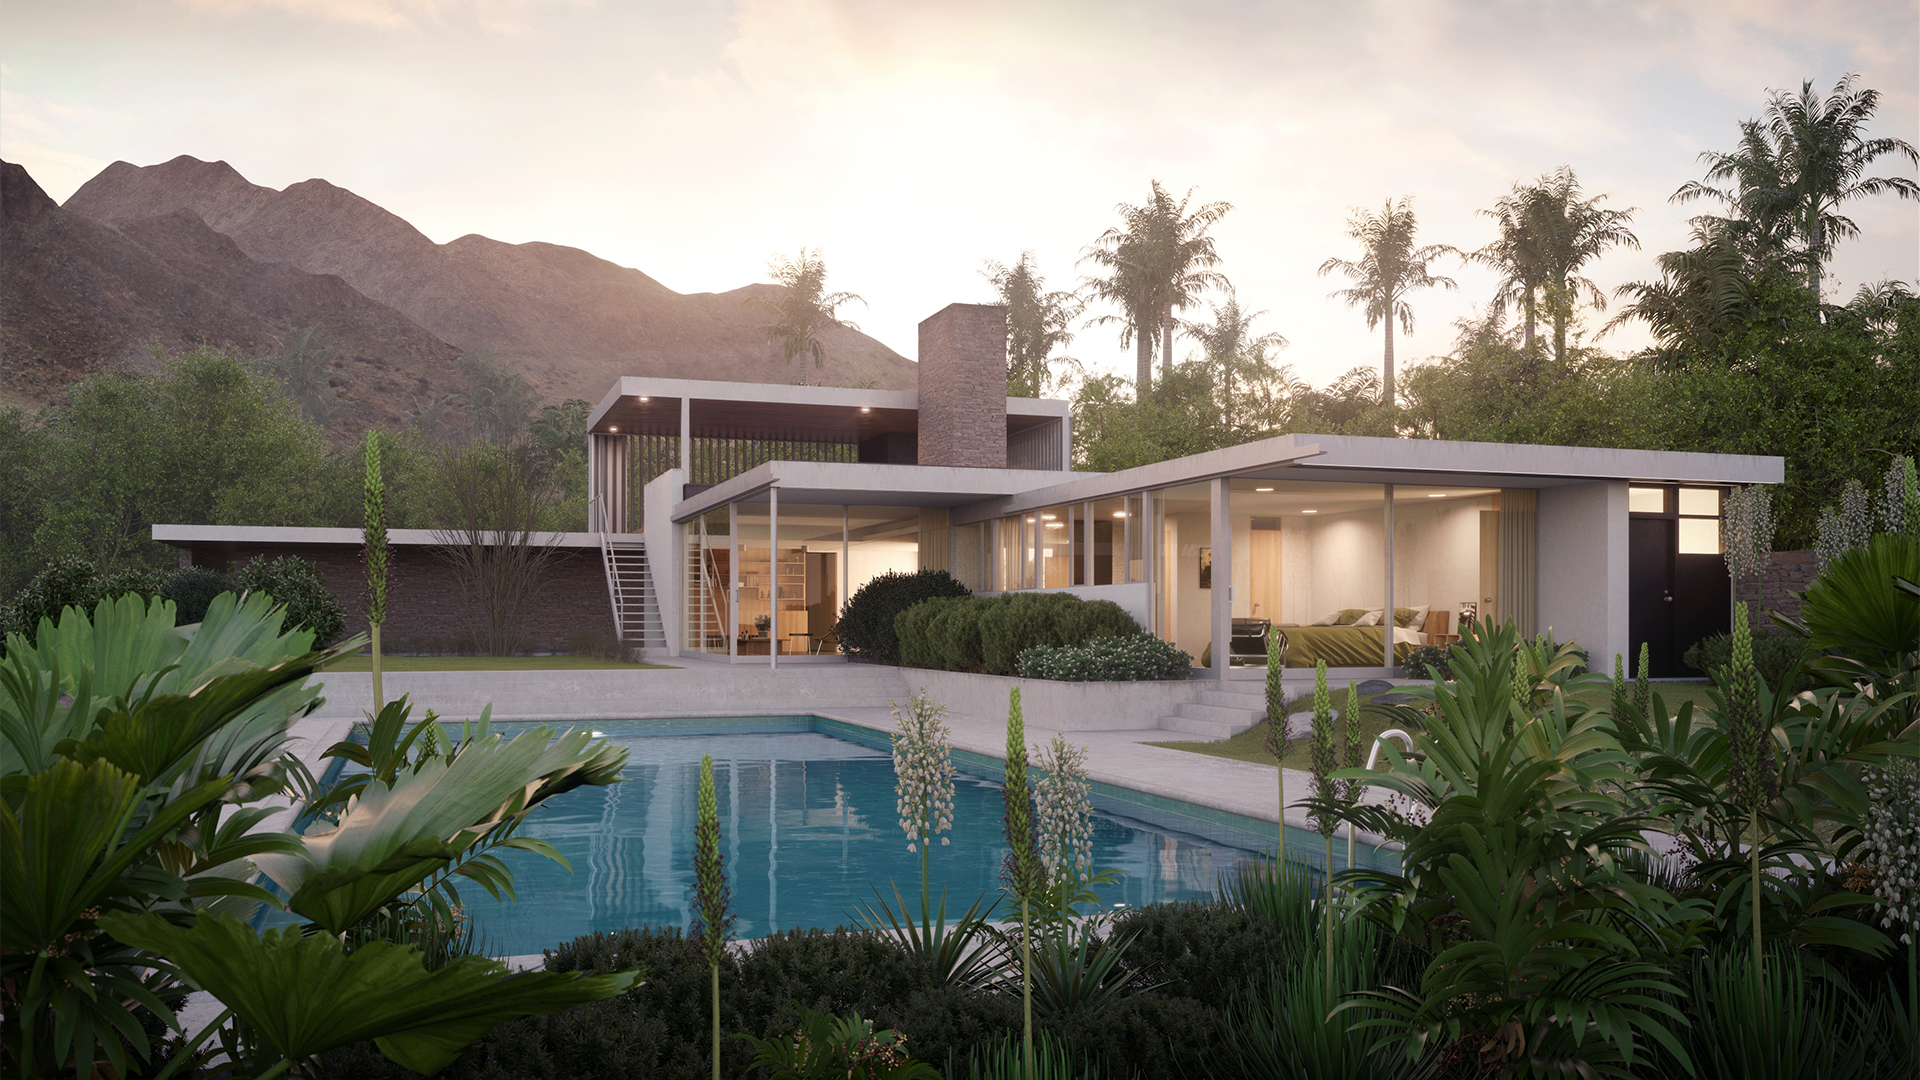
\includegraphics[width=\textwidth,height=\textheight,keepaspectratio]{images/1_introduction/Laubwerk-Kit-12_Bauclassroom-Exterior.jpg}
  \caption{An example of a complex scene created by Laubwerk Plants Kits, extracted from \cite{laubwerk}}
  \label{fig:intro_complexScene}
\end{figure}

After a scene is created and rendered, all the hard work invested by the artist 
is stored, waiting for a possible future use. However, should the artist choose 
to change renderers, the scene file they created so diligently would have to be 
rewritten and/or heavily modified.

Converting a scene file from one renderer format to another is very difficult and time consuming. Unfortunately, the various rendering systems available use proprietary scene description formats. Aside from adapting material and light properties - which can be hard since sometimes renderers don't provide the same features -, the 3D object formats supported may not be the same. Manually converting a scene from one format to the other can extremely time consuming, taking up to several days per scene. \cite{tungsten}


\section{Improving PBR}

Currently, PBR and MC Ray Tracing are the only practical solution for simulating global illumination effects in complex environments. Due to its high computational cost, an image can take a long time to render - sometimes up to a few days, depending on the complexity of the scene or the technique used. This means that it is practically impossible to use these images in real-time applications.

There are some techniques that aim to improve the time spent rendering PBR images, like improved sampling~\cite{Heck2013, Pilleboue:2015} and reconstruction strategies~\cite{Sen2012, Rousselle2013, Kalantari2015, Bitterli2016}. These techniques are implemented on top of an existing PBR system as a way of using aspects of the MC Ray Tracing algorithm (such as ray-object intersection calculations) that are orthogonal to the proposed methods.

Since converting scenes between renderers is a strenuous, time-consuming task, these new techniques are often constrained to demonstrate their results on a limited set of scenes available for the chosen renderer. This apparently simple limitation has profound implications, as it constrains a direct comparison between MC rendering techniques that have been implemented using different rendering systems.

\section{Project Definition}	

We present {\it a system for automatic conversion among scene file formats used by PBR systems}. Our solution intends to expand the repertoire of scenes available for testing, validation, and benchmarking of PBR algorithms. Currently, our system handles conversions among PBRT v3, Mitsuba, and LuxRender, which are three of the most popular physically-based renderers. 

Extending it to support additional renderers is straightforward. Our solution (discussed in Section~\ref{sec:systemarch}) consists of {\it importing} any source scene description into a canonical representation, which can then be {\it exported} to 
other scene formats. 

\begin{figure*}[h]
  \centering
  \subfloat[PBRT v3]{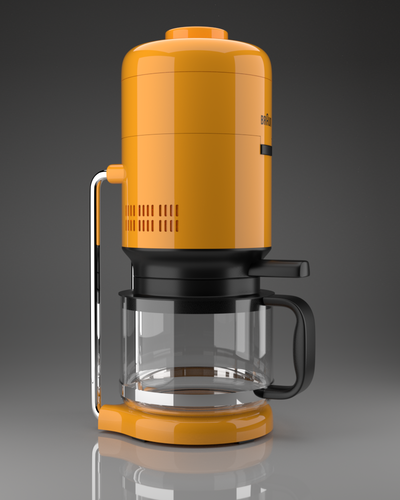
\includegraphics[width=0.33\linewidth]{images/5_results/coffee/1_from_pbrt.png}
	  \label{breakfast_Lux}	
  }	
  \subfloat[Mitsuba]{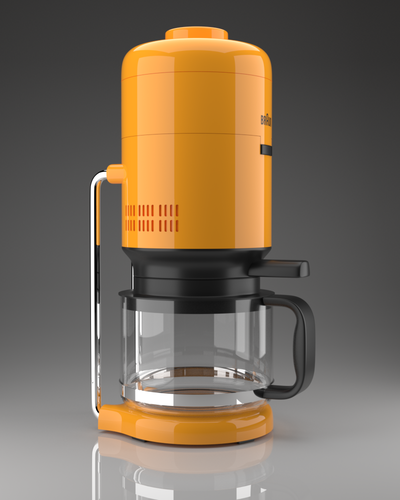
\includegraphics[width=0.33\linewidth]{images/5_results/coffee/2_to_mitsuba.png}
	  \label{breakfast_PBRT}		
  }	
  \subfloat[LuxRender]{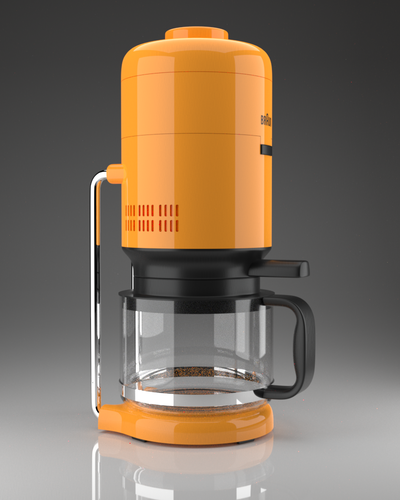
\includegraphics[width=0.33\linewidth]{images/5_results/coffee/3_to_lux.png}
		  \label{breakfast_Mitsuba}	
  }	
  \caption{Example of automatic scene conversion obtained with our system. \textit{Coffee Maker} rendered with PBRT v3 (left). Rendering produced by Mitsuba (center) and LuxRender (right), using converted scenes (from PBRT v3) for these rendering systems.}
  \label{fig:teaser}
\end{figure*}

Figure~\ref{fig:teaser} illustrates the use of our system to perform automatic conversion of a scene represented in the PBRT v3 format. The images at the center and on the right show, respectively, the renderings produced by Mitsuba and by LuxRender, from converted scenes files. Note the correct representation of the various materials (glass, plastic, and metal).

Our work does not introduce a new physically-based rendering technique per se. Instead, it falls in the area of {\it meta-research} systems, which are systems 
designed to facilitate and improve the research process. Meta-research systems are quite common in computer graphics and computer vision~\cite{MiddleburyStereo, MiddleburyFlow, AlphaMatting, VideoMatting}, where they have led to significant progress in these fields. 
  
Recently, \cite{Santos:2018:FBKSD} introduced a framework for developing and benchmarking MC sampling and denoising algorithms. This is achieved by providing an API that decouples the developed techniques from the used rendering system. 

While it allows a technique to be tested on any rendering system that supports the proposed API, each rendering system is still constrained to a limited set of test scenes. Our system is orthogonal to and complements this API, aspiring to reach full orthogonality among algorithms, rendering systems and scene files.

The {\bf contents} of our work include:
\begin{itemize}
	\item A system for automatic conversion among scene file formats used by Monte Carlo physically-based rendering systems (Chapter~\ref{sec:systemarch}).
	It enables algorithms implemented on different rendering systems to be tested on similar scene descriptions, giving developers and end user a better 
assessment of the strengths and limitations of MC rendering techniques;
	\item The proposal of a mechanism intending to achieving orthogonality among MC rendering algorithms, rendering systems and scene files (Chapter~\ref{sec:systemarch}). 
This could be achieved when integrated with the API provided in~\cite{Santos:2018:FBKSD}. 
\end{itemize}

\section{Contents of this Report}

This work includes a detailed description of how our solution for converting scenes between renderers was implemented, from system architecture to result 
images and analysis.

We discuss, in chapter \ref{sec:related_work}, similar systems developed as meta-reseach, such as other attempts to convert scenes and exporting a generic 
scene format into different renderer-specific outputs. Following the current state-of-the-art, we delve a little into the history of rendering in chapter \ref{sec:theory}, starting with the first algorithms and then moving on to currently used physically-based renderers.

Our system is described in chapter \ref{sec:systemarch}, where we explain how our pipeline works and how we converted some renderer-specific directives. In the next chapter, as a closing demonstration. we show some results obtained from scene files converted by our system.


